\section{Sampling 采样}

\Paragraph{Perfect Sampling 完美采样}

\begin{paracol}{2}
    
    The in-situ stresses on a clay element are usually anisotropic, in that the horizontal and vertical stresses are not equal. Prior to running a laboratory triaxial shear test, the clay must of course be removed from the ground, taken to the lab, trimmed, and finally mounted in the test apparatus. The term perfect sampling denotes this process where no disturbance has been given to the specimen other than that involved with the release of the in-situ shear stresses.

    \switchcolumn

    黏土单元上的原位应力通常是各向异性的,因为水平应力和垂直应力不相等。 在进行实验室三轴剪切试验之前,当然必须将黏土从地面上移走,送到实验室,修整,最后安装在试验设备中。 术语“完美采样”表示此过程,除了释放原位剪应力外,没有对样品产生干扰。

    \switchcolumn*

    The ratio of horizontal to vertical effective stress in a one dimensionally consolidated horizontal clay deposit is denoted by $K_0=\overline\sigma_{hc}/\overline\sigma_{cc}$. For normally consolidated clays, $K_0$ has been found by \citet{Bishop19582} and \citet{Simons1958} to agree substantially with \citet{Jaky1948103} expression for the $K_0$ of granular systems, that is,$K_0 = 1-sin\overline{\phi}$, where $\overline{\phi}$ equals the friction angle at maximum obliquity. For overconsolidated clays, $K_0$ increases with irmreasing overconsolidation ratio (OCR=$\overline\sigma_{vm}/\overline\sigma_{vc}$ ratio of maximum past to existing vertical consolidation pressures).  \citet{Skempton1961351}  found for the highly plastic London clay that $K_0$ reached unity at an OCR of about 2.2 and attained values of 2 to 3 at an OCR exceeding about 8.

    \switchcolumn

    一维固结水平黏土沉积物中水平有效应力与垂直有效应力之比用$K_0=\overline\sigma_{hc}/\overline\sigma_{cc}$表示。 对于正常固结的黏土,\citet{Bishop19582}和\citet{Simons1958}发现$K_0$与\citet{Jaky1948103}表示的粒状系统$K_0$基本吻合,即$K_0 = 1-sin\overline{\phi}$  ,其中$\overline{\phi}$等于最大倾角时的摩擦角。 对于超固结黏土,$K_0$随超固结比的增加而增加(OCR=$\overline\sigma_{vm}/\overline\sigma_{vc}$过去的最大值与现有垂直固结压力的比值)。 \citet{Skempton1961351} 发现,对于高塑性伦敦黏土,$K_0$的OCR约为2.2时达到了单位,而OCR超过约8时达到了2到3的值。

    \switchcolumn*

    The isotropic effective stress after perfect sampling, $\overline{\sigma}_{ps}$, of a saturated clay which had in-situ vertical and horizontal consolidation pressures of $\overline{\sigma}_{v0}$ and $K_0\overline{\sigma}_{v0}$, respectively, is given by

    \switchcolumn

    原位垂直和水平固结压力分别为$\overline{\sigma}_{v0}$和$K_0\overline{\sigma}_{v0}$的饱和黏土的完美采样后的各向同性有效应力$\overline{\sigma}_{ps}$由下式给出

\end{paracol}

\begin{align}
    \overline{\sigma}_{ps}=\overline{\sigma}_{v0}\left[K_0+A_u(1-K_0)\right]
    \label{equation:1}
\end{align}

\begin{paracol}{2}
    
    \noindent{}where $A_u=(\Delta_u-\Delta\sigma_h)/(\Delta\sigma_v-\Delta\sigma_h)=$ an A parameter\footnote{
        A is defined in terms of horizontal and vertical stresses in order to be consistent with the definition of $K_0$, Skempton's B parameter \citep{Skempton1954143} is taken equal to unity. 为了与$K_0$的定义一致,根据水平和垂直应力定义A,Skempton的B参数等于1。} 
    for the undrained release of the shear stresses which existed at the K0 condition by changing the horizontal and vertical stresses in order to achieve an isotropic stress system.

    \switchcolumn

    \noindent{}式中$A_u=(\Delta_u-\Delta\sigma_h)/(\Delta\sigma_v-\Delta\sigma_h)=$为了实现各向同性的应力系统,通过改变水平和垂直应力,$K_0$条件下存在的不释放剪应力的参数A。

    \switchcolumn*

    The relationship between $\overline{\sigma}_{ps}$ and $\overline{\sigma}_{v0}$ is illustrated in \autoref{figure:1} for normally consolidated (Point A) and highly overconsolidated (Point B) specimens of a hypothetical clay for three different values of $A_u$. The straight line from the origin to Point A indicates a constant $K_0$ of 0.65 for normally consolidated clay; the curved line from point A to Point B shows an increasing value of Ko as the OCR increases ($K_0=2.2$ for OCR = 10 at Point B). The figure shows that $\overline{\sigma}_{ps}/\overline{\sigma}_{v0}$ for normally consolidated clay will always be less than unity for $A_u$ values less than one; the reverse is true for overconsolidated specimens with $K_0>1$, that is, $\overline{\sigma}_{ps}/\overline{\sigma}_{v0}$ will be greater than unity for Au values less than one.

    \switchcolumn

    对于三种不同的$A_u$值,假设黏土的正常固结(A点)和高度固结(B点)样品的$\overline{\sigma}_{ps}$和$\overline{\sigma}_{v0}$之间的关系如\cnfigureref{figure:1}所示。 从原点到A点的直线表明,对于正常固结的黏土,$K_0$的常数为0.65; 从点A到点B的曲线显示,随着OCR的增加,$K_0$的值也随之增加(对于B点处的OCR = 10,$K_0=2.2$)。 该图表明,对于正常固结的黏土,当$A_u<1$时$\overline{\sigma}_{ps}/\overline{\sigma}_{v0}$始终小于1。 反之适用于$K_0\geq{}1$的超固结试样,即,当$A_u<1$时,$\overline{\sigma}_{ps}/\overline{\sigma}_{v0}$将大于1。
    
\end{paracol}

\begin{figure}[!htb]
    \centering
    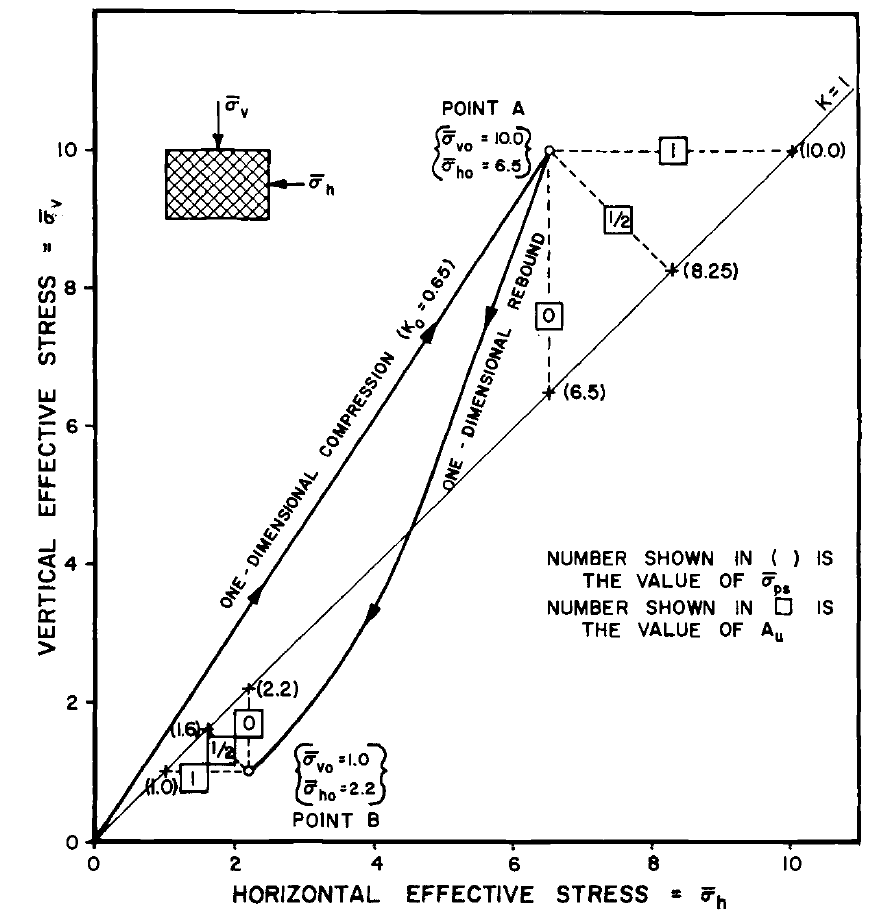
\includegraphics[width=0.5\textwidth]{figures/figure-1.png}\\
    The one-dimensional compression and rebound curves simulate $K_0$ data for the London clay \citet{Skempton1961351}. \\
    一维压缩和回弹曲线模拟了伦敦黏土citet{Skempton1961351}的$K_0$数据。
    \caption{Perfect Sampling of a Normally Consolidated Clay and an Over-consolidated Clay.}
    \addtocounter{figure}{-1}
    \vspace{-5pt}
    \renewcommand{\figurename}{图}
    \caption{正常固结土和超固结土的完美采样。}
    \renewcommand{\figurename}{Figure}
    \label{figure:1}
\end{figure}

\begin{paracol}{2}
    
    \autoref{figure:2} illustrates the effects of perfect sampling on stress paths for a group of clays from Kawasaki, Japan. Pairs of specimens were normally consolidated second specimen was first unloaded by decreasing the axial pressure (that is, perfect sampling), and then loaded by increasing the axial pressure with both steps being done under undrained conditions with pore pressure measurements ($CA-\overline{UU}$ test). The resulting values of the ratio $\overline{\sigma}_{ps}/\overline{\sigma}_{1c}$ were $0.56\pm{}0.05$ with corresponding $A_u$ values of $0.17\pm{}0.10$. Similar test data on normally consolidated Boston Blue Clay (plasticity index = 14 percent; $K_0\approx{}0.54$) yielded $\overline{\sigma}_{ps}/\overline{\sigma}_{1c}=0.59$ and $A_u= 0.11$.

    \switchcolumn

    \cnfigureref{figure:2}说明了完美采样对一组来自日本Kawasaki的黏土的应力路径的影响。 成对的样品通常是固结的,第二个样品首先通过降低轴向压力来卸载(即完美采样),然后通过在不排水条件下利用孔隙压力测量($CA-\overline{UU}$试验)完成两个步骤来增加轴向压力来进行加载 。$\overline{\sigma}_{ps}/\overline{\sigma}_{1c}$之比的所得值为$0.56\pm{}0.05$,相应的$A_u$值为$0.17\pm{}0.10$。 在正常固结的波士顿蓝黏土上的类似试验数据(塑性指数=$14\%$; $K_0\approx{}0.54$)得出$\overline{\sigma}_{ps}/\overline{\sigma}_{1c}=0.59$和$A_u= 0.11$。

\end{paracol}

\begin{figure}[!htb]
    \centering
    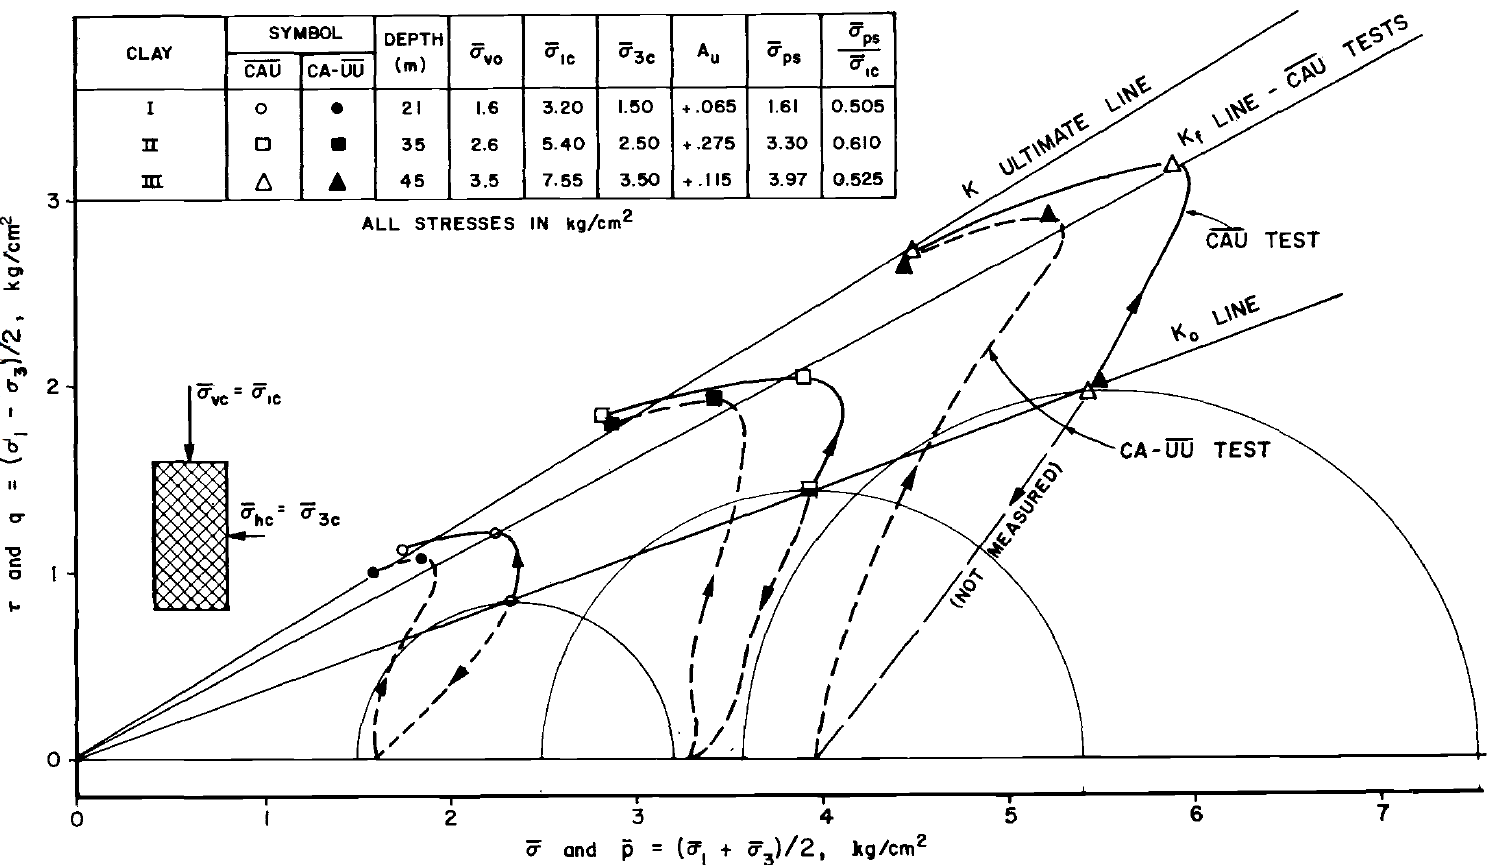
\includegraphics[width=0.8\textwidth]{figures/figure-2.png}
    \caption{Effect of Perfect Sampling on Stress Paths for Normally Consolidated Kawasaki Clays.}
    \addtocounter{figure}{-1}
    \vspace{-5pt}
    \renewcommand{\figurename}{图}
    \caption{完美采样对正常固结的川崎黏土应力路径的影响。}
    \renewcommand{\figurename}{Figure}
    \label{figure:2}
\end{figure}

\begin{paracol}{2}
    
    What are thought to be typical values of $K_0$, $A_u$, and $\overline{\sigma}_{ps}/\overline{\sigma}_{v0}$ are suggested in \autoref{table:1} based on the above and other rather limited data by \citet{Bishop195394} and \citet{Skempton1961351}. As shown in \autoref{table:1}, the effective stress of perfect samples will be only 35 to 80 percent of the in-situ vertical effective stress $\overline{\sigma}_{v0}$ for normally consolidated clays, but may be double $\overline{\sigma}_{v0}$ for a highly overconsolidated plastic clay.

    \switchcolumn

    在\cntableref{table:1}中,根据\citet{Bishop195394}和\citet{Skempton1961351}的上述以及其他相当有限的数据,在\cntableref{table:1}中提出了被认为是$K_0$,$A_u$和$\overline{\sigma}_{ps}/\overline{\sigma}_{v0}$的典型值。 如表一所示,对于正常固结的黏土,理想样品的有效应力仅为原位垂直有效应力的35$\%$至80$\%$,而对于高度超固结的塑料黏土,其有效应力可能是$\overline{\sigma}_{v0}$的两倍。

\end{paracol}

\begin{table*}[!htb]
    \centering
    \caption{STRESS RATIOS FOR PERFECT SAMPLING.}
    \addtocounter{table}{-1}
    \vspace{-8pt}
    \renewcommand{\tablename}{表}
    \caption{完美采样的应力比。}
    \vspace{4pt}
    \renewcommand{\tablename}{Table}
    \begin{tabularx}{\textwidth}{XXXX}
        \toprule
        Type of Specimen & $K_0$ & $A_u$ & $\overline{\sigma}_{ps}/\overline{\sigma}_{v0}$ \\
        \midrule
        Normally consolidated & & & \\
        ~~Clayey Silt & 0.4 to 0.5 & -0.1 to 1 & 0.35 to 0.5 \\
        ~~Lean Clay & 0.5 to 0.6 & ~0.1 to 0.2 & 0.55 to 0.7 \\
        ~~Plastic Clay & 0.6 to 0.7 & ~0.2 to 0.3 & 0.65 to 0.8 \\
        Heavily overconsolidated & & & \\
        ~~Plastic Clay & $\sim$2.5 & $\sim$0.3 & $\sim$2 \\
        \bottomrule
    \end{tabularx}%
    \label{table:1}%
\end{table*}


\Paragraph{Actual Sampling 实际采样}

\begin{paracol}{2}
    
    The ideal sampling process would involve neither a change in moisture content nor a change in magnitude and distribution of effective stresses upon removing a specimen of clay from the field and placing it in the shear test equipment. Such sampling is essentially impossible and the best that can be hoped for is what has been termed in this paper perfect sampling, that is, the removal of the shear stresses acting on the element in tile field to achieve the isotropic stress $\overline{\sigma}_{ps}$. The effects of perfect sampling on the undrained shear behavior in triaxial compression of a normally consolidated clay were illustrated in \autoref{figure:2}.

    \switchcolumn

    理想的采样过程既不涉及水分含量的变化,也不涉及在从现场中取出黏土样本并将其放置在剪切试验设备中时有效应力的大小和分布的变化。 这样的采样基本上是不可能的,可以期望的最好是本文中所称的完美采样,即消除作用在瓷砖场中元素上的剪应力,以实现各向同性应力$\overline{\sigma}_{ps}$。 理想采样对正常固结黏土三轴压缩中不排水剪切行为的影响如\cnfigureref{figure:2}所示。

    \switchcolumn*

    The actual sampling process offers many opportunities for additional disturbance of the soil structure according to \citet{Rutledge19441155}, \citet{Hansen1948189} and \citet{Hvorslev1949}. Some of these effects are illustrated in \autoref{figure:3}, which presents a hypothetical stress path for an element of normally consolidated clay during tube sampling. The Point P with an effective stress of $\overline{\sigma}_{ps}$, corresponds to perfect sampling, whereas Point G with an effective stress of $\overline{\sigma}_r$ represents the effective stress of an actual specimen at the start of a UU shear test. It is proposed that the ratio $\overline{\sigma}_r/\overline{\sigma}_{ps}$ is a measure of the amount of additional disturbance caused by actual sampling.

    \switchcolumn
   
    根据\citet{Rutledge19441155},\citet{Hansen1948189}和\citet{Hvorslev1949}的说法,实际的采样过程为土壤结构的其他扰动提供了许多机会。 其中一些效果如\cnfigureref{figure:3}所示,它为试管采样过程中正常固结的黏土元素提供了假设的应力路径。 有效应力为$\overline{\sigma}_{ps}$的点P对应于完美采样,而有效应力为$\overline{\sigma}_r$的点G表示在UU剪切试验开始时实际样品的有效应力。 建议比率$\overline{\sigma}_r/\overline{\sigma}_{ps}$是对实际采样引起的附加干扰量的度量。

\end{paracol}

\begin{figure}[!htb]
    \centering
    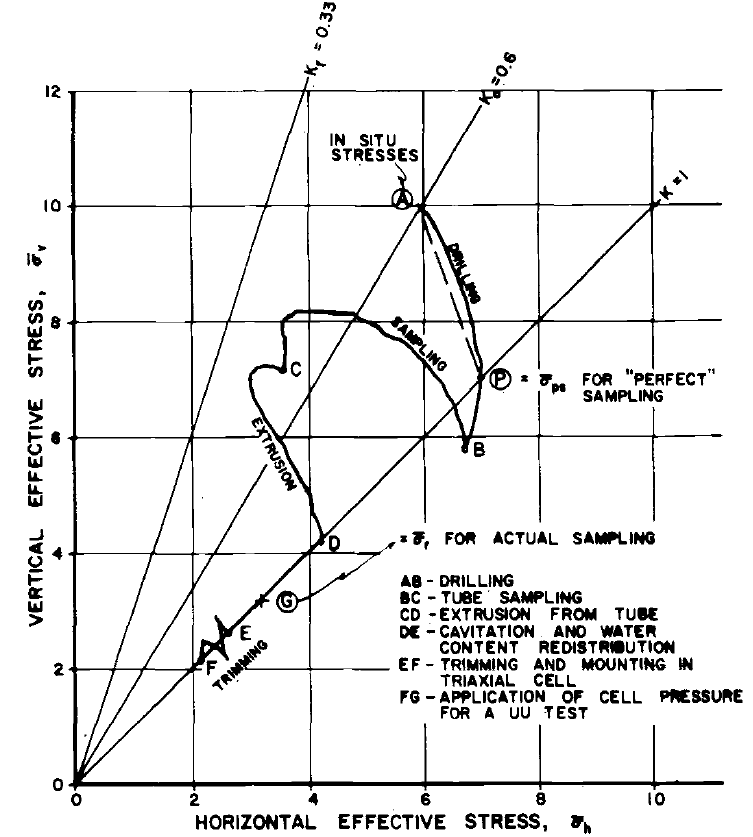
\includegraphics[width=0.5\textwidth]{figures/figure-3.png}
    \caption{Hypothetical Stress Path for a Normally Consolidated Clay Element During Tube Sampling.}
    \addtocounter{figure}{-1}
    \vspace{-5pt}
    \renewcommand{\figurename}{图}
    \caption{管道采样期间正常固结黏土单元的假设应力路径。}
    \renewcommand{\figurename}{Figure}
    \label{figure:3}
\end{figure}

\begin{paracol}{2}
    
    Measured values of the residual effec tive stress after sampling, $\overline{\sigma}_r$, are presented in \cnfigureref{figure:4} for an overconsolidated deposit of Boston Blue Clay and for normally consolidated strata of Kawasaki clays (see \cntableref{table:2} for further data on these clay deposits). The apparatus for UU tests described in the next section was used to measure $\overline{\sigma}_r$ with a total chamber pressure generally between 1 and 3 $\rm{kg/cm^2}$, for which the B parameter became essentially equal to unity. Values of the maximum past pressure, $\overline{\sigma}_{vm}$, in-situ vertical effective stress, $\overline{\sigma}_{v0}$, and effective stress for perfect sampling, $\overline{\sigma}_{ps}$,, are shown for comparison. The ratio $\overline{\sigma}_r/\overline{\sigma}_{ps}$, which is proposed as a measure of the degree of excessive disturbance, ranged from 0.11 to 0.43 with an average value of 0.28 for the Kawasaki clays. Values of $\overline{\sigma}_r/\overline{\sigma}_{ps}$ for the deposit of Boston Blue Clay, which ranged from 0.01 to 0.34, showed a marked decrease with increasing depth and decreasing overconsolidation ratio. Partial drying of the deepest specimen of Boston Blue Clay (depth = 26.2m) revealed a grossly distorted structure which corroborates the very low value of $\overline{\sigma}_r$ of only 0.02 $\rm{kg/cm^2}$. Data from two UU tests on normally consolidated Lagunillas clay (case B in \autoref{table:2}) yielded values of $\overline{\sigma}_r/\overline{\sigma}_{ps}$, equal to $0.36\pm{}0.07$.

    \switchcolumn

    \cnfigureref{figure:4}给出了波士顿蓝黏土超固结沉积物和Kawasaki黏土正常固结地层的采样后残余有效应力的测量值$\overline{\sigma}_r$(有关这些黏土沉积物的更多数据,请参见\cntableref{table:2})。 下一节中描述的用于UU测试的设备用于测量总腔室压力$\overline{\sigma}_r$,通常在1-3$\rm{kg/cm^2}$之间,对于该腔室,B参数基本上等于1。为了比较,显示了最大过去压力$\overline{\sigma}_{vm}$,原位垂直有效应力$\overline{\sigma}_{v0}$和完美采样的有效应力$\overline{\sigma}_{ps}$的值。作为对过度扰动程度的一种度量,提出的比率$\overline{\sigma}_r/\overline{\sigma}_{ps}$在0.11至0.43的范围内,Kawasaki黏土的平均值为0.28。 波士顿蓝土沉积物的$\overline{\sigma}_r/\overline{\sigma}_{ps}$值在0.01到0.34之间,随深度增加和过固结率降低而显着降低。波士顿蓝黏土的最深标本(深度为26.2m)的部分干燥显示出严重扭曲的结构,这证实了其仅0.02$\rm{kg/cm^2}$的非常低的$\overline{\sigma}_r$值。 在正常固结的Lagunillas黏土上进行的两次UU测试数据(\cntableref{table:2}中的情况B)得出的$\overline{\sigma}_r/\overline{\sigma}_{ps}$值等于$0.36\pm{}0.07$。

\end{paracol}

\begin{figure}[!htb]
    \centering
    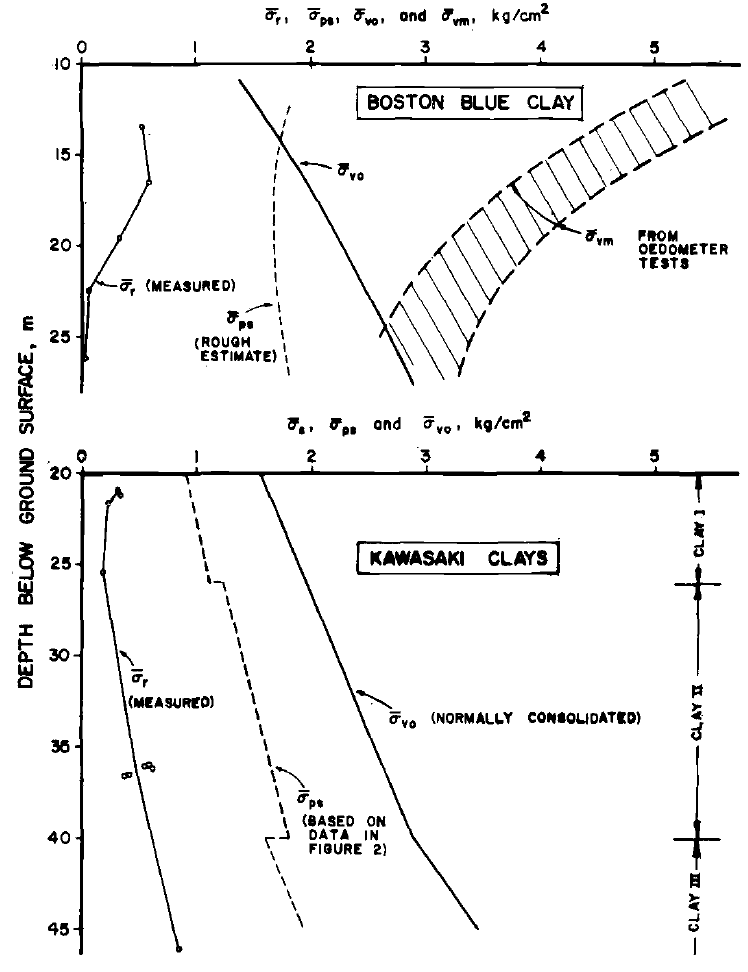
\includegraphics[width=0.5\textwidth]{figures/figure-4.png}
    \caption{Effect of Tube Sampling on Effective Stresses for Boston Blue Clay and the Kawasaki clays.}
    \addtocounter{figure}{-1}
    \vspace{-5pt}
    \renewcommand{\figurename}{图}
    \caption{采样对波士顿蓝黏土和川崎黏土有效应力的影响。}
    \renewcommand{\figurename}{Figure}
    \label{figure:4}
\end{figure}

\begin{table}[!htb]
    \centering
    \scriptsize
    \renewcommand{\arraystretch}{1.2}
    \caption{COMPARISON OF UNDRAINED STRENGTH FROM UU AND CU TESTS.}
    \addtocounter{table}{-1}
    \vspace{-8pt}
    \renewcommand{\tablename}{表}
    \caption{UU和CU试验的不排水强度的比较。}
    \vspace{4pt}
    \renewcommand{\tablename}{Table}
    \begin{threeparttable}[b]
        \setlength{\tabcolsep}{0.4mm}{
        \begin{tabularx}{\textwidth}{lllllllll}
            \toprule
             & & & & \multicolumn{2}{l}{From U or UU Tests} & & & \\
            Case & Location & Description of Clay & Depth, m & $S_u, \rm{kg/cm^2}$ & $S_u/\overline{\sigma}_{v0}$ & $\dfrac{S_u(UU)}{S_u(CIU,\overline{\sigma}_c=\overline{\sigma}_{v0})}$ & Remarks & Source \\
            \midrule
            A & \makecell[tl]{M.I.T., \\~~Cambridge,\\~~Mass}             & \makecell[tl]{o.c.\tnote{a} a Boston blue clay\\o.c. Boston blue clay \\~~~~~~(slightly)\\n.c.\tnote{b} Boston blue clay} & \makecell[tl]{12.2\\18.3\\\\27.4} & \makecell[tl]{0.80\\0.68\\\\0.50} & \makecell[tl]{0.59\\0.37\\\\0.185} & \makecell[tl]{~~0.74\\~~0.77\\\\~~0.58} & \makecell[tl]{3 in. diameter shelby \\~~fixed piston samples} & M.I.T.\\
            B & \makecell[tl]{Lagunillas, \\~~Venezuela}               & \makecell[tl]{n.c. plastic clay \\~~$w_L\cong{}61\%$ \\~~$P.I.\cong{}37\%$} & 6.2 & 0.18 & 0.30 & ~~0.75 & \makecell[tl]{3 in. diameter shelby samples.\\~~$S_u$(UU) based on average \\~~of U and UU data} & M.I.T. \\
            C & \makecell[tl]{Kawasaki, \\~~Japan}                     & \makecell[tl]{normally consolidated \\~~plastic clay \\~~Clay I, P.I.\tnote{c}$\cong{}31\%$\\~~Clay I, P.I. $\cong{}36\%$\\~~Clay II, P.I.$\cong{}43\%$} & \makecell[tl]{\\\\20.5\\25\\35} & \makecell[tl]{\\\\0.50\\0.49\\0.69} & \makecell[tl]{\\\\0.31\\0.26\\0.27} & \makecell[tl]{\\\\~~0.64\\~~0.58\\~~0.57} & \makecell[tl]{3 in. diameter shelby samples.\\~~$S_u$(UU) from top one-third \\~~of U and from UU data \\~~corrected to $t_f=5$ hr} & M.I.T. \\
            D & \makecell[tl]{Gulf of \\Mexico}                          & \makecell[tl]{o.c. soft plastic clay\\~~P.I.$\cong{}80\%$\\~~L.I.$\cong{}50\%$\\firm plastic clay with silt \\~~and sand\\~~P.L.$\cong{}60\%$\\~~L.I.$\cong{}35\%$} & \makecell[tl]{0 to 6 \\\\\\18 to 50} & \makecell[tl]{avg.$\cong{}$0.27\\\\\\acg.$\cong{}$0.50} & \makecell[tl]{...\\\\\\...} & \makecell[tl]{$\sim{}$0.85\\\\\\$\sim{}$0.5} & Shelby samples & \citet{Fenske195616} \\
            E & \makecell[tl]{Skabo, Oslo,\\~~Norway}                  & \makecell[tl]{n.c. plastic clay with a \\~~high salt content\\~~P.I. $\cong{}30\%$\\~~L.I.$\cong{}65\%$\\~~$S_t\cong{}30\%$} & 10.6 to 16 & avg.=0.32 & 0.31 & ~~0.74 & \makecell[tl]{2.1 in. diameter thin walled\\~~fixed piston samples} & \makecell[tl]{N.G.I. Internal\\~~Report No.\\~~F175 (1962)}\\
            F & \makecell[tl]{$\rm{G\ddot{o}ta}$ Valley, \\~~Sweden}   & \makecell[tl]{Lilla Edet Clay\\~~highly  o.c. P.I. $\cong{}30\%$\\~~slightly o.c. P.I.$\cong{}33\%$\\~~slightly o.c. P.I.$\cong{}29\%$\\~~slightly o.c. P.I.$\cong{}37\%$} & \makecell[tl]{\\~~~4 to 6.8\\~~10 to 12.3\\16.2 to 18\\10.8 to 12.8} & \makecell[tl]{\\avg.$\cong{}$0.4\\avg.=0.34\\avg.=0.46\\avg.=0.13} & \makecell[tl]{\\$\sim$1.20\\~~0.45\\~~0.42\\~~0.13} & \makecell[tl]{\\$\sim$0.90\\~~0.60\\~~0.66\\~~0.40} & \makecell[tl]{2.1 in. diameterr thin walled \\~~fixed piston samples. Clay \\~~believed to have a significant \\~~amount of natural \\~~cementation} & \begin{minipage}[t]{1.6cm}\citet{Bjerrum1960101}\end{minipage} \\
            G & \makecell[tl]{Mexico City}                             & \makecell[tl]{Mexico City CLay, \\~~slightly o.c.} & ... & ... & ... & ~~0.74 & ... & \citet{Marsal1957229}\\
            H & \makecell[tl]{Drammen, \\~~Norway}                     & \makecell[tl]{normally consolidated soft \\~~silty clay with thin seams \\~~of silt and fine sand\\~~P.I.$\cong{}8\% S_t=10$\\~~P.I.$\cong{}16\% S_t=9$\\~~P.I.$\cong{}14\% S_t=9$} & \makecell[tl]{\\\\\\~5\\12\\18} & \makecell[tl]{\\\\\\0.25\\0.25\\0.24} & \makecell[tl]{\\\\\\0.37\\0.19\\0.24} & \makecell[tl]{\\\\\\~~0.97\\~~0.57\\~~0.40} & \makecell[tl]{2.1 in. diameter thin walled, \\~~fixed piston samples. $S_u$\\~~(UU) based on U samples \\~~with lowest strain at failure} & \citet{Simons1960727}\\
            I & \makecell[tl]{Sault Ste.\\~~Marir, Mich}               & \makecell[tl]{n.c. varved clay\\~~P.I.$\cong{}28\%$\\~~$S_t\cong{}8$} & $\sim$9 & $\sim$0.3 & $\sim$0.15 & $\sim$0.60 & \makecell[tl]{3.5 in. diameter thin walled \\~~piston. $S_u$(CIU) based on \\~~$S_u/\overline{\sigma}_c$ for $\overline{\sigma}_c>\overline{\sigma}_{v0}$} & \begin{minipage}[t]{1.4cm}\citet{Wu19581, Wu19621}\end{minipage}\\
            \bottomrule
        \end{tabularx}}%
        \begin{tablenotes}
            \item[a] O.C. = overconsolidated.
            \item[b] N.C. = normally consolidated.
            \item[c] P.I. = plasticity index.
        \end{tablenotes}
    \end{threeparttable}  
    \label{table:2}%   
    \renewcommand{\arraystretch}{1.0}
\end{table}


\begin{paracol}{2}
    
    These limited data show that the effective stress of laboratory specimens of normally consolidated and slightly overconsolidated clays after tube sampling may be lowered by excessive disturbance to a value of only $20\pm20$ percent of the theoretical value for perfect sampling. It is therefore suggested that the measurement of the residual effective stress, $\overline{\sigma}_r$, of laboratory specimens should become a standard test for jobs requiring a rational interpretation of lab strength data, especially for deep tube samples of normally consolidated clay. The value of $\overline{\sigma}_r$ can be obtained from a direct measurement of the residual pore pressure $u_r$, (that is, $u$ at zero confining pressure; \cite{Lambe1961207} describes several methods for measuring $u_r$) provided that $\overline{\sigma}_r$ is less than one atmosphere, although the use of a confining pressure of several atmospheres is preferable since the B parameter is generally some-what less than unity.\footnote{
        In this case UU tests with a confining pressure sufficient to make B equal unity are preferable to unconfined compression tests. 在这种情况下,UU试验的围压足以使B等于1,优于无限制压缩试验。
    } \citet{Skempton1961351} suggests some indirect methods for evaluating $\overline{\sigma}_r$.

    \switchcolumn

    这些有限的数据表明,由于过度扰动,正常固结和稍固结的粘土的实验室标本的有效应力可能会由于过度干扰而降低,仅为理想采样的理论值的$20\%\pm{}20\%$。 因此,建议对于需要合理解释实验室强度数据的工作,特别是对于通常固结的粘土的深管样品,对实验室样品的残余有效应力$\overline{\sigma}_r$的测量应成为标准测试。$\overline{\sigma}_r$的值可以通过直接测量残余孔隙压力$u_r$(即$u$在零围压下; \cite{Lambe1961207}描述了几种测量$u_r$的方法)获得,前提是$\overline{\sigma}_r$小于一个大气压,尽管最好使用几个大气压的限制压力,因为B参数通常略小于1。\citet{Skempton1961351}提出了一些间接的方法来评估$\overline{\sigma}_r$。

    \switchcolumn*

    Experience at Massachusetts Institute of Technology has shown, for example, that the size of the specimen, the amount of trimming, and the placement of the specimen in an oedometer ring can affect the value of $\overline{\sigma}_r$. In other words, the value of $\overline{\sigma}_r$, and hence the degree of disturbance, are really variables.

    \switchcolumn

    麻省理工学院的经验表明,例如,标本的大小,修整量以及标本在里程表环中的放置都会影响$\overline{\sigma}_r$的值。 换句话说,$\overline{\sigma}_r$的值以及扰动程度实际上是变量。

\end{paracol}